\documentclass{article}[jsarticle]
\setlength{\parindent}{0pt}
\usepackage[T1]{fontenc}
\usepackage[dvipdfmx]{hyperref}
\usepackage{lmodern}
\usepackage{latexsym}
\usepackage{amsfonts}
\usepackage{amssymb}
\usepackage{mathtools}
\usepackage{nccmath}
\usepackage{amsthm}
\usepackage{multirow}
\usepackage{graphicx}
\usepackage[dvipdfmx]{color}
\usepackage{wrapfig}
\usepackage{here}
\usepackage{float}
\usepackage{ascmac}
\usepackage{url}
\usepackage{listings}
\usepackage{xcolor}
\usepackage{pifont}
\usepackage{appendix}

\lstset{
    basicstyle=\ttfamily\color{white},
    numbers=none,  % Line numbers
    numberstyle=\tiny\color{white},
    numbersep=5pt,
    tabsize=2,
    extendedchars=true,
    breaklines=true,
    keywordstyle=\color[rgb]{0.58,0.00,0.83},
    stringstyle=\color[rgb]{0.81,0.36,0.00},
    identifierstyle=\color{white},
    commentstyle=\color[rgb]{0.34,0.62,0.16},
    rulecolor=\color[rgb]{0.5,0.5,0.5},
    xleftmargin=0.1cm,    % Left margin
    xrightmargin=0.1cm,   % Right margin
    language=python,
    backgroundcolor=\color[rgb]{0.13,0.13,0.13},
    showspaces=false,
    showstringspaces=false
}



\title{特別研究3 研究報告書}
\author{高林秀 \\ 三宅研究室 博士前期課程2年 \\ V-CampusID : 23vr008n}
\date{\today}

\begin{document}

\maketitle

\begin{abstract}
    \noindent
    本稿は2024年度特別研究3の研究報告書である。前半は研究テーマの概要と説明を、後半は7月31日現在の研究進捗状況を報告するものである。\par
    \noindent
    特別研究3(以下、本研究と呼称)では、昨年度特別研究2まで行っていた「自律航行ドローンによる物資輸送アプローチの検討」から研究課題を変更し、
    『津波避難誘導の「マルチエージェント強化学習」とドローンによるアプローチの検討』とした。\par 
    \noindent
    % TODO本稿内容の要約
\end{abstract}

\tableofcontents

\section{研究課題について}
本章では、本研究における研究課題の説明と、背景、新規性、最終目標について述べる。
\subsection{概要説明}
\paragraph{研究課題}
\begin{center}
    \textbf{津波避難誘導のマルチエージェント強化学習ドローンによるアプローチの検討}
\end{center}
以下、本研究のポイントをまとめる。
\begin{itemize}
    \item 大規模な群衆の津波避難誘導をマルチエージェント強化学習により最適化、機械化を目指す.
    \item 津波避難タワーや津波避難ビルへ避難者を誘導し、制限時間以内で避難率の最大化を目指す
    \item MARL、ゲームAIの災害対応への応用可能性の検証。
\end{itemize}
観光地や沿岸部地域における津波避難の誘導を行うエージェントモデルをマルチエージェント強化学習(以下、MARL)により構築することを目的とする。\par
エージェントはドローンとし、大規模な群衆を複数のドローンによる誘導を行うことで、避難率の最大化を目指す。\par
また、シミュレーションで構築した強化学習モデルを組み込んだ実機でのプロトタイプ制作を行い、実際の運用時における課題や問題点を洗い出す。

昨年度特別研究2までは、『自律航行ドローンによる物資輸送アプローチの検討』を行っていたが、以下の事由により研究課題を上記に変更した。
\begin{itemize}
    \item 強化学習によるアプローチの不適切性
    \item 強化学習により、最適化する指標が不明確であり研究課題として成立しない
\end{itemize}

\subsection{研究背景}
本研究を行う背景と意義について述べる。\par 
大きな背景としては、特別研究1および特別研究2で記載した報告書と同じであるため詳細については、そちらを参照されたい。(特別研究1,2の研究報告書については、付録のURLに添付する)。
ここでは、簡潔に記載するに留める。\par

\paragraph{機械化へのニーズ}
津波に限らず、災害時の避難誘導においては二次被害のリスクを大きく伴う。実際、2011年に発生した東日本大震災では、地元住民の避難誘導に当たっていた警察官の方々が多数殉職するなどの被害も起きている。
この実態について、詳しくは後述の\hyperref[sec:research-sec1]{『我が国における津波避難の課題についての調査』}にて取り上げる。 \par
そういった二次被害を無くし、安全に避難誘導を行うための研究が官民連携で、近年盛んに行われている背景がある。
例えば、東日本大震災で大きな津波被害を受けた宮城県仙台市では、自治体と民間企業が連携し、災害発生状況の確認や避難指示を行うドローンの実証実験が2018年に行われた.
\begin{figure}[H]
    \centering
    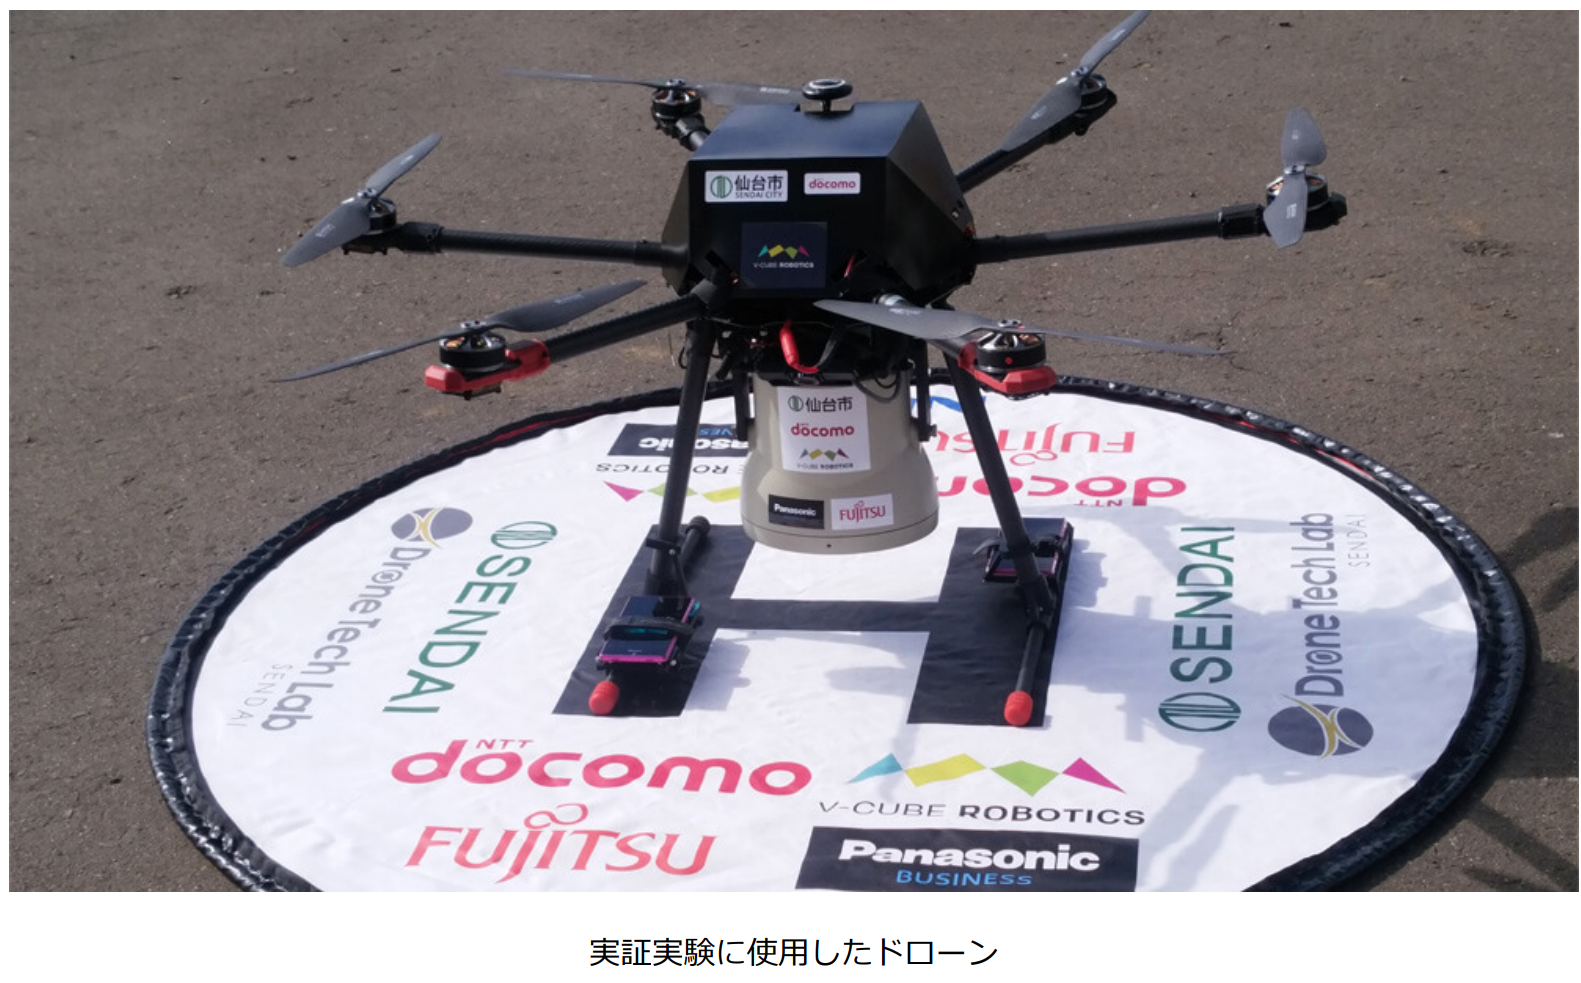
\includegraphics[scale=0.5]{./images/drone1.png}
    \caption{
       仙台市と複数の民間企業の実験で使用されたドローン \\
    【引用元】:富士通ジャーナル『ドローンで津波避難誘導、被災状況をリアルタイムで把握』 2018.04.12 \\
    }
    \url{https://www.fujitsu.com/downloads/JP/microsite/fujitsutransformationnews/journal-archives/pdf/2018-04-12-01.pdf}
\end{figure}

\paragraph{災害対応人材の不足}
災害大国である我が国において, 被災者の捜索, 被害状況の把握,救援物資の現地輸送といった対応は, 迅速かつ効率的に行われなければならない.
しかし近年, そのような災害対応を一任務とする, 自衛隊員の人材が不足している,あるいは今後さらに不足する事態が予想されている。
そのような背景に加え、自衛隊におけるドローン配備の増強と活用も近年大きく進められた。陸上自衛隊東部方面総監部とJUIDA(日本UAS 産業振興
協議会)
\footnote{一般社団法人日本UAS 産業振興協議会 JUIDA: 我が国における無人航空機の産業振興を目的に
2014 年 7 月に設立された. 無人航空機の情報周知活動や, 航行ガイドラインの策定, 市場創造支援な
どに取り組んでいる.
3
}
が大規模災害発生時における相互協力を目的とした協定を締結しており,今後自衛隊の災害派遣においてドローンの利活用がさらに進むことが予想される.


\paragraph{航空法改正とレベル4飛行の解禁}
レベル4 飛行とは, 有人地帯での目視外飛行のこと. 目視で監視できない状態で, 有人地帯上空を自律飛行することができる飛行レベルを指
す. 我が国では2022年12月5日に改正航空法が施行され, レベル4 飛行が解禁された\cite{art1}[2].
これにより, 現在ドローンの災害対応における有効性に注目が集まっている.
\begin{figure}[H]
    \centering
    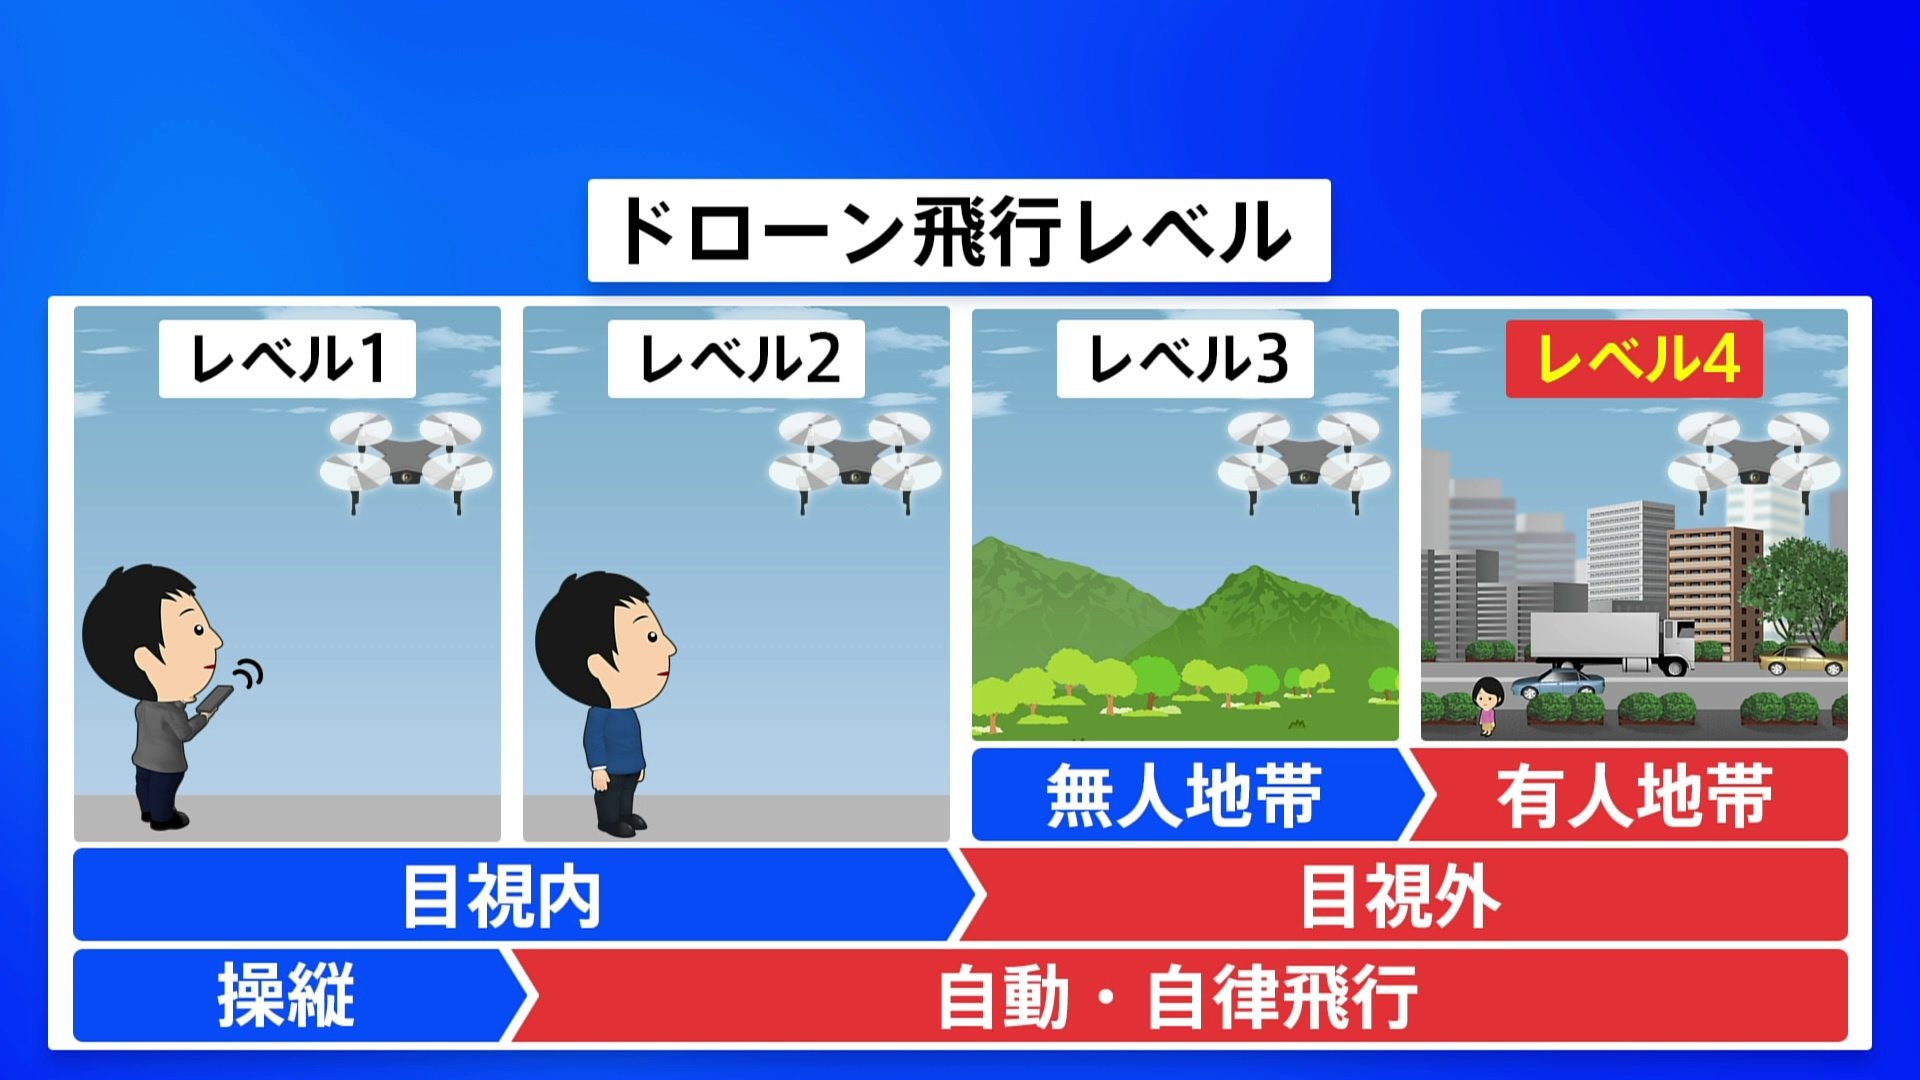
\includegraphics[scale=0.2]{./images/img_e2902b05dd2c63b869ea3d4f75a4c2e3350873.jpg}
    \caption{
       レベル4 飛行について \\
    【引用元】: TBS 報道資料 2022.12.15 \\
    }
    \url{https://newsdig.tbs.co.jp/articles/-/221701}
\end{figure}

\subsection{新規性・最終目標}
本研究の新規性については、以下の点を挙げる事ができる。
\begin{itemize}
    \item ドローンの防災活用自体まだまだ新しい分野。
    \item 複数機が連携した運用 \& AI, 強化学習訓練の導入事例が無い。
    \item 都市モデルを活用した訓練環境の構築
\end{itemize}
都市モデルについては、正確性,再現性の観点から、国土交通省がオープンソースで開発、提供しているPLATEAU(プラトー)\footnote{PLATEAU は、国土交通省が主導する日本全国の3D都市モデルの設備・オープンデータ化プロジェクトである。データ形式はCityGMLを基本とし、他にも様々なデータ形式に変換したものを配布している}を利用する。
また、研究の最終目標については以下を想定している。
\begin{itemize}
    \item ドローン誘導の有無による避難率の変化の検証
    \item MARLドローンの災害対応への応用可能性を示す。
    \item 現実空間で動かし、プロトタイプ制作を行う。
\end{itemize}

\section{これまでの取り組み}
本章では、2024年7月31日現在までの本研究における取り組み、各種調査状況、開発状況について述べる。
\subsection{調査関係}
本研究を行う上で、津波避難時の課題や、先行研究、類似研究が無いかについて調査を行った。その結果を以下順に記載する。
\subsubsection{我が国における津波避難の課題についての調査}
\label{sec:research-sec1}
%TODO: ここに調査結果を記載

\subsection{シミュレーション・実験関係}
本研究では、シミュレーションを用いたモデル開発を行う。その開発状況について以下に記載する。
なお開発には、Unity/C\#とその深層強化学習ライブラリであるML\-Agentsを使用している。\par 
なお、詳細な仕様については付録記載の別資料を参照されたい。

\subsubsection{簡易シミュレータの開発と実験}
大規模な都市モデルを用いた開発の前に、事前準備、テスト開発として簡易なゲーム空間におけるシミュレーションを2種類開発した。
\begin{enumerate}
    \item フィールド上に避難者と避難タワーがランダムな位置に生成される。
    \item エージェントは制限時間内に避難者をタワーに誘導するタスクを解く
    \item チーム全体の報酬として、エージェントが誘導した避難者数を報酬とし、その最大化を目指す。
    \item この時、避難者が自身のみでタワーまで到達した場合、その分は報酬から除外する。
\end{enumerate}

\paragraph{フラット環境}
この環境は下図のように、単純な平面3D空間において、ドローンによる津波避難タワーへの誘導を試験、シミュレーションする環境である。
\begin{figure}[H]
    \centering
    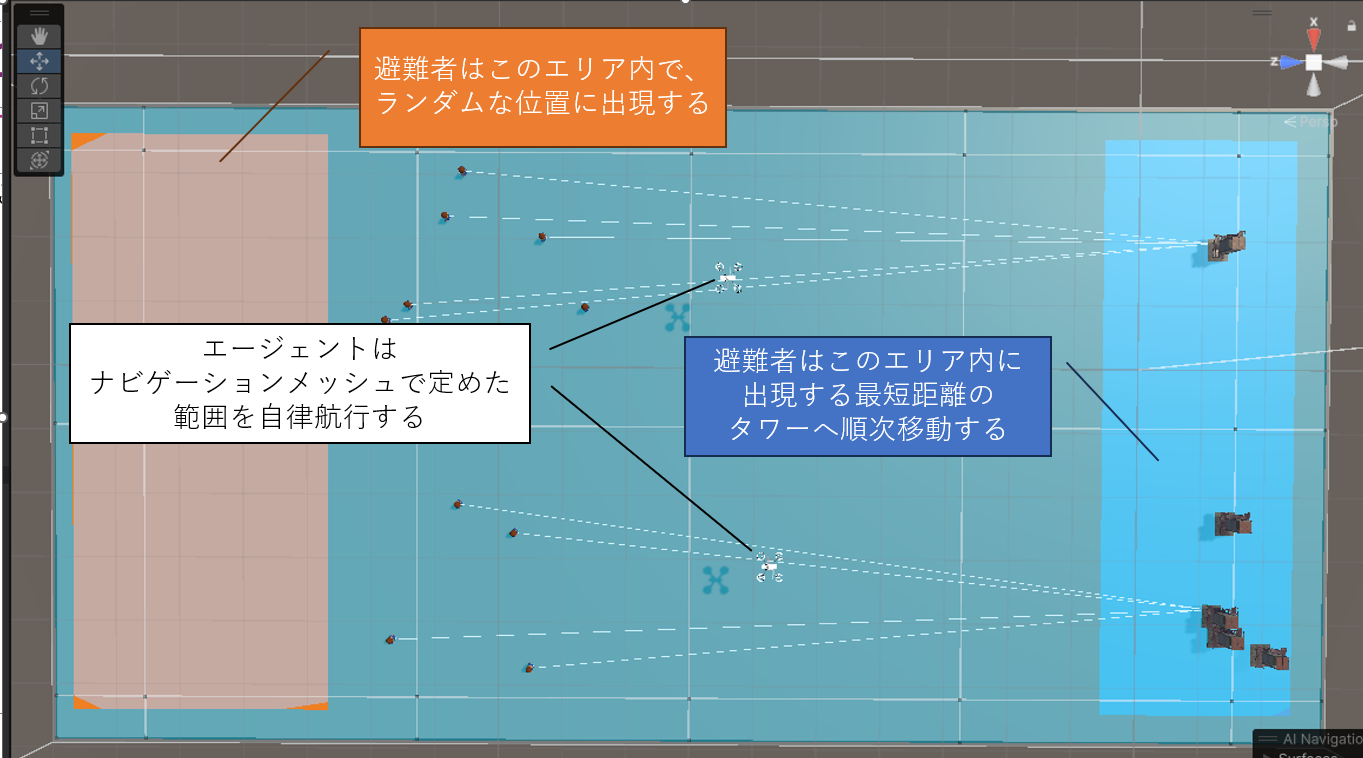
\includegraphics[scale=0.3]{./images/FIeld-3.png}
    \caption{
       開発したフラット環境の全貌図
    }
\end{figure}

\paragraph{障害物フラット環境}
前述したフラット環境の避難者経路上にランダムに障害物を生成した環境での実験を行った。
\begin{figure}[H]
    \centering
    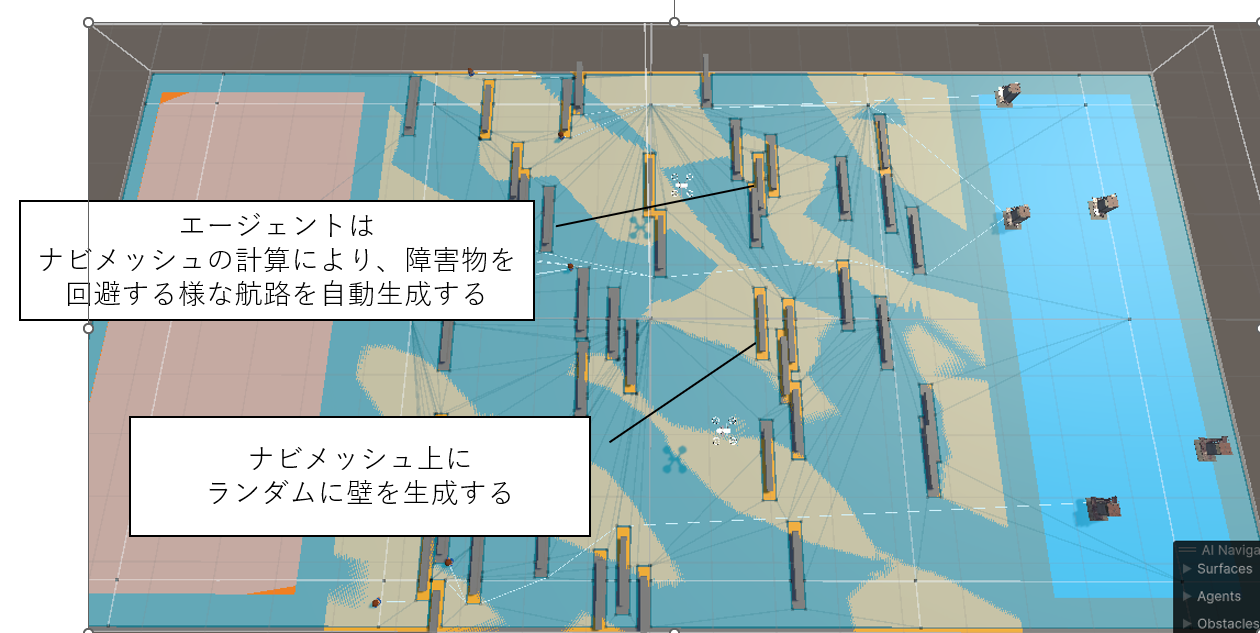
\includegraphics[scale=0.3]{./images/Field-4.png}
    \caption{
       開発した障害物フラット環境の全貌図
    }
\end{figure}

学習実行中の様子はそれぞれ以下のようになる。
%TODOフラット環境の学習実行中の画像


\paragraph{実験結果}
実験の結果以下のような結果が得られた。
\begin{itemize}
    \item どちらの環境も、92000stepあたりから徐々にエージェントが避難者を誘導するようになった。
    \item 個別報酬、全体報酬ともに、ステップ毎でバラつきはあるものの、徐々に増加する傾向が見られ、エージェントが避難者をタワーまで誘導するタスクを学習できることを確認した。
\end{itemize}
\begin{figure}[H]
    \centering
    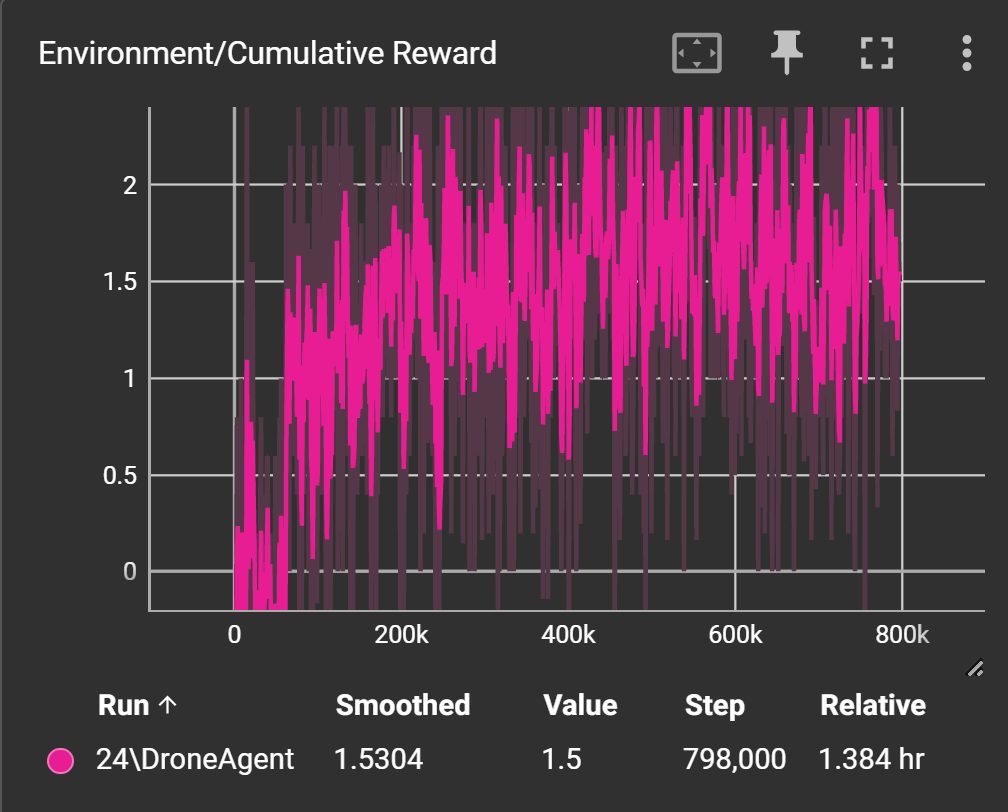
\includegraphics[scale=0.6]{./images/result-1.png}
    \caption{
       エージェント毎の報酬の推移
    }
\end{figure}
\begin{figure}[H]
    \centering
    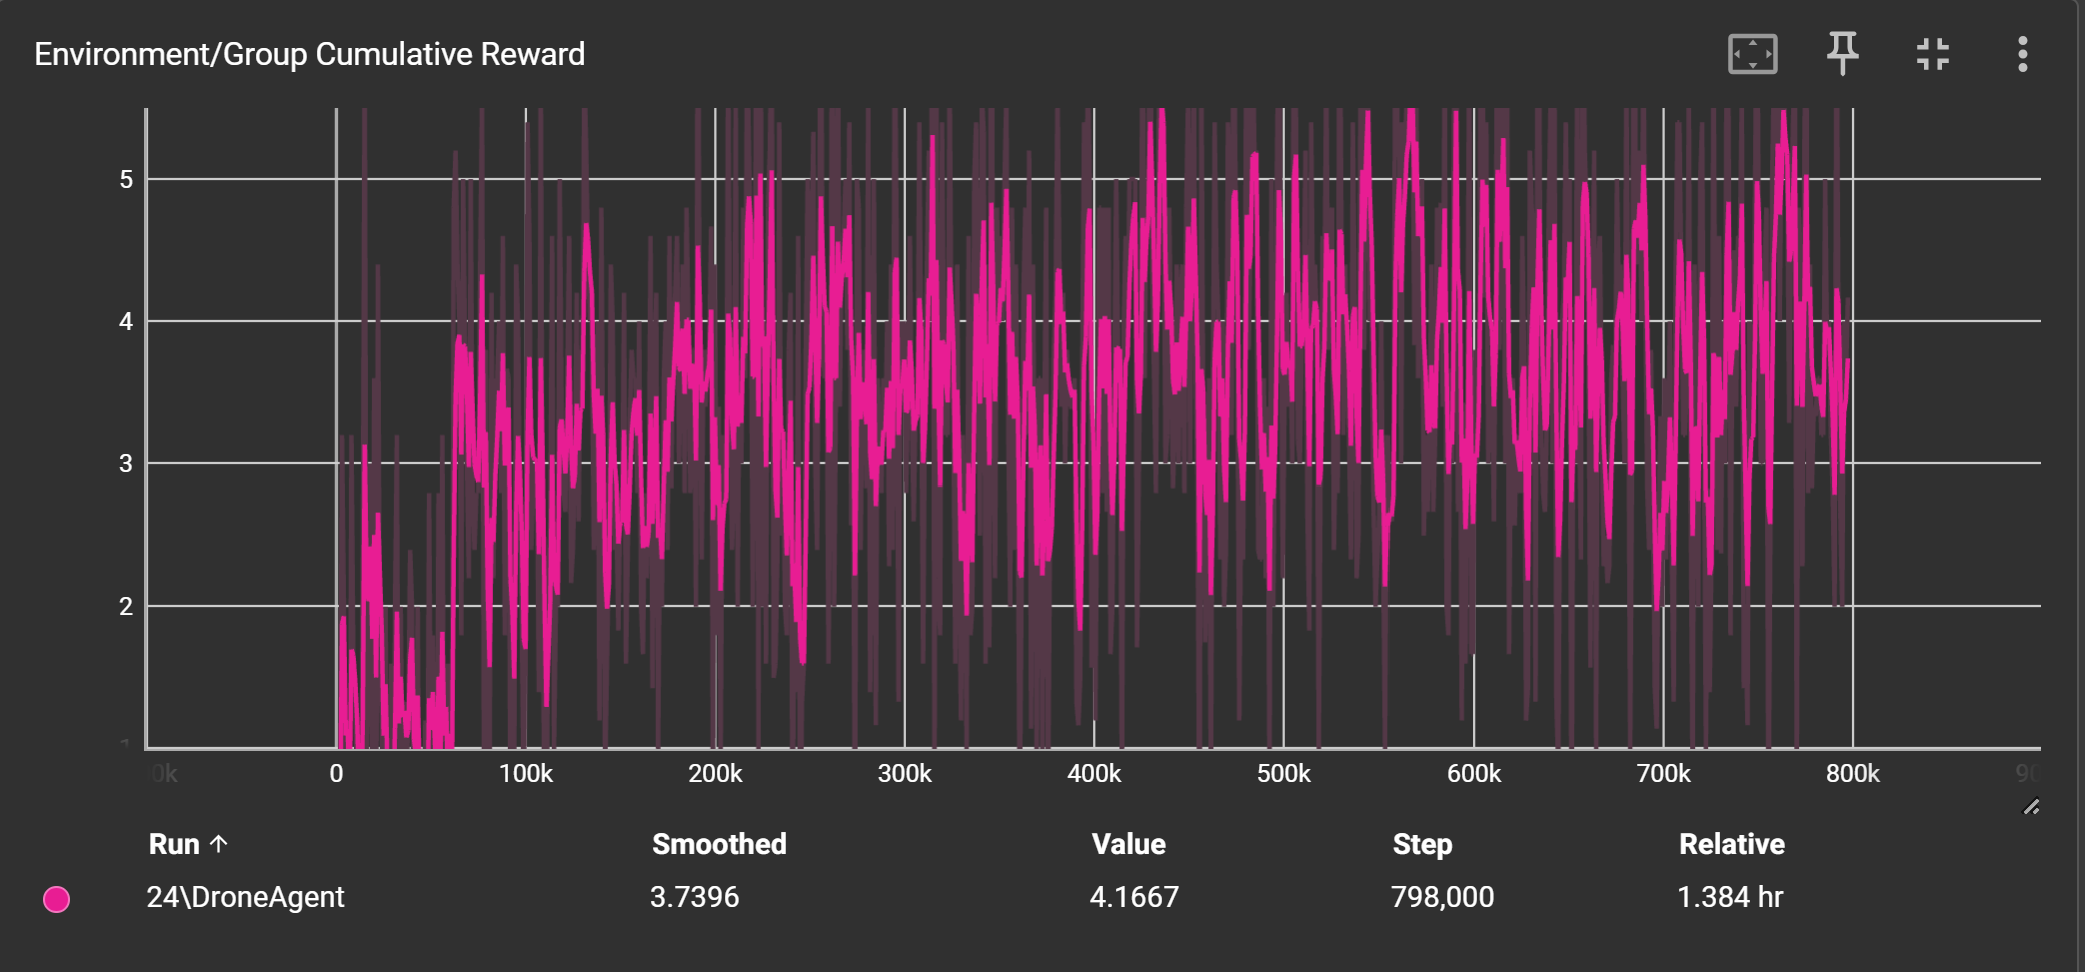
\includegraphics[scale=0.4]{./images/result-2.png}
    \caption{
       全体報酬の推移
    }
\end{figure}

しかし、実験を進める中で以下のような課題も発見した。
\begin{itemize}
    \item 長時間(7000k step)学習させると、エージェントが避難者を誘導せず、タワーまで先回りして報酬を獲得してしまう。
    \item 誘導すべき避難者がまだ存在しているが、エージェントが次のタワーまで移動してくれない。(複数人、追加の誘導ができていない)
    \begin{itemize}
        \item 上記の問題は、エージェントの報酬が2,3付近で頭打ちになってしまっていることからも確認できる。
    \end{itemize}
\end{itemize}
また、全体的に報酬は右肩上がりではあるものの、ステップ毎の報酬の差が大きく、安定して学習が進んでいるとは言い難い状況である。

\subsubsection{都市モデルでのシミュレーション}
PLATEAUを用いた都市モデルを活用したシミュレーション環境の開発も行った。津波避難ビルの指定は、実際のハザードマップを参考に推定し実装した。
\begin{itemize}
    \item エージェントの移動可能範囲は、道路上空のみとした。
    \item 市が認定の津波避難ビルを避難所対象(4か所の津波避難ビル)
    \item 観光客や通行人等、屋外にいる人を避難者として想定
\end{itemize}
\begin{figure}[H]
    \centering
    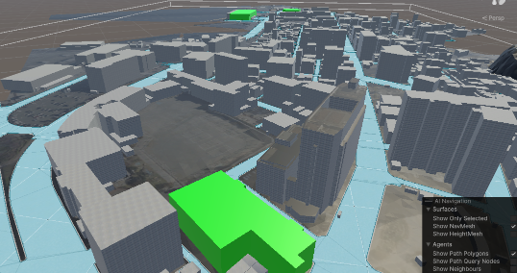
\includegraphics[scale=0.8]{./images/PLATEAU-demo.png}
    \caption{
       横須賀市のPLATEAUモデルを用いた環境
    }
\end{figure}
なお、現状強化学習環境としては未完成である。現状、都市モデルでの環境構築は以下の課題を抱えており、これらの解決に向け尽力している。
\begin{itemize}
    \item 避難者の初期生成位置が指定の場所よりがズレる
    \item ナビメッシュ上のカーブ、交差点部分で避難者が動作しなくなる
\end{itemize}

現状実装している都市モデルのシミュレーションは、横須賀市のみであるが、修士論文に向けて以下の都市モデルも追加予定である。
\begin{itemize}
    \item 静岡県沼津市
    \item 福島県南相馬市
\end{itemize}


\section{現在の進捗状況}
\subsection{進捗状況まとめ}

\subsection{現在の課題}

\section{修士論文に向けて}

\begin{thebibliography}{9}
    \bibitem{art1} 航空法等の一部を改正する法律案を閣議決定, 国土交通省, 2021 年, \url{https://www.mlit.go.jp/report/press/kouku01_hh_000110.html}
\end{thebibliography}

\begin{appendix}
    \paragraph{特別研究1 研究報告書} \par
    \url{}

    \paragraph{特別研究2 研究報告書} \par
    \url{}

    \paragraph{シミュレーション仕様詳細資料} \par 
    \url{}

    \paragraph{開発リポジトリ} \par
    本研究の開発コード等は、以下のGitHubリポジトリにて公開している。
    \url{https://github.com/tsyu12345/Rikkyo-MasterPJ}

\end{appendix}

\end{document}